\subsection{Experimental Settings}

\subsubsection{Datasets}
We conducted experiments using the CVC-ClinicDB dataset \cite{BERNAL201599} and the Kvasir-SEG dataset \cite{jha2020kvasir}.
The CVC-ClinicDB dataset consists of $612$ colonoscopy images ($384 \times 288$ pixels), and the Kvasir-SEG dataset consists of $1000$ colonoscopy images.
Both datasets are comprised of colonoscopy images and their corresponding ground truth polyp masks.
The data was split using 5-fold cross-validation.
For the CVC-ClinicDB dataset, we used GroupKFold splitting to ensure that frames from the same video sequence did not span across different folds.

\subsubsection{Implementation Details}
We adopted U-Net \cite{ronneberger2015u} with the architecture shown in Table \ref{tab:unet_architecture} as the segmentation model.
We used the Adam optimizer \cite{kingma2014adam} for training, with the batch size set to $32$ and the learning rate set to $10^{-3}$.
As preprocessing, all images were resized to $W = 224$ pixels and $H = 224$ pixels.
During training, we applied horizontal/vertical flips and brightness/contrast adjustments with a probability of $50\%$.
The maximum number of epochs $E$ was set to $200$.

Uncertainty estimation via MC Dropout was performed every $\tau=10$ epochs.
Dropout layers were placed in the final block of the encoder and the final block of the decoder.
During each evaluation, based on previous work \cite{pmlr-v48-gal16},
we performed $T = 10$ stochastic inferences with a dropout rate of $p = 0.5$.
Additionally, the percentile for normalizing the difficulty metric within the dataset was set to $q = 25$ considering the skewness of the difficulty distribution.
Based on the results of preliminary experiments, the start epoch for adaptive learning was set to $E_0 = 10$, with $\epsilon_{\text{min}}=0$, $\epsilon_{\text{max}}=0.5$, 
and $k=2$.\subsubsection{Comparison Conditions}To evaluate the effectiveness of adaptive learning, we compare the proposed method with the following methods:

\begin{itemize}
    \item Dice Loss \cite{milletari2016v}: A standard loss function in medical image segmentation, adopted as the baseline.
    \item Focal Loss \cite{lin2017focal}: A method that addresses class imbalance by down-weighting the loss of easy samples.
    It shares a common motivation with the proposed method in terms of  ``weighting according to sample difficulty''.
    However, the difference lies in that Focal Loss uses static weighting based on prediction confidence,
    whereas the proposed method uses dynamic weighting based on model uncertainty.
    The rate for down-weighting easy samples was set to $\gamma = 2$.
    \item PolyDice-1 Loss ($\epsilon = 0$): The standard form of PolyDice-1 Loss, which theoretically approximates the standard Dice Loss.
    It was adopted as a reference to verify the pure effect of manipulating the parameter $\epsilon$ in comparison with the proposed method and the Optimal setting described below.
    \item PolyDice-1 Loss (optimal): To evaluate the theoretical upper bound of performance with a fixed $\epsilon$,
    we retrospectively searched for the $\epsilon$ value that maximizes the Dice coefficient on the test data
    and included this as an ideal setting for comparison. Specifically,
    we exhaustively evaluated $\epsilon$ in the range of $\{-0.3, -0.2, \ldots, 0.5\}$
    and determined the value $\epsilon$ that achieved the highest accuracy for each dataset.
    Although this setting is impossible to realize in practical operation,
    it represents the performance under the ideal condition where the ``optimal fixed value is known beforehand''.
\end{itemize}

Through these comparisons, we verify: (1) whether the proposed method is superior to standard loss functions,
(2) whether adaptive $\epsilon$ control is more effective than fixed $\epsilon = 0$, and (3) whether the proposed method can achieve performance comparable to or exceeding the optimal setting.

\subsubsection{Evaluation Metrics}
To evaluate segmentation performance, we used the Dice coefficient and IoU(Intersection over Union) to measure region overlap, 
and precision and recall to measure detection accuracy.
Let $\tilde{Y}_n = \{\tilde{y}_{n,i,j}\}$ be the predicted mask obtained by binarizing the model's prediction map
$\hat{\mathbf{Y}}_n$ for image $n$ with a threshold $\theta_\text{th} = 0.5$.
The numbers of true positive (TP), false positive (FP), and false negative (FN) pixels for image $n$ are defined as follows:
\begin{align}
    TP_n &= \sum_{j=1}^{W} \sum_{i=1}^{H} \tilde{y}_{i, j} y_{i, j} \text{,}\\
    FP_n &= \sum_{j=1}^{W} \sum_{i=1}^{H} \tilde{y}_{i, j} (1 - y_{i, j}) \text{,}\\
    FN_n &= \sum_{j=1}^{W} \sum_{i=1}^{H} (1 - \tilde{y}_{i, j}) y_{i, j} \text{,}
\end{align}

\begin{itemize}
    \item Dice coefficient: Evaluates the overlap between the ground truth and predicted regions directly.
    It was adopted as the main metric because it can appropriately reflect the extraction accuracy of minute objects even in unbalanced images like medical images.
    \begin{align}
        \text{Dice}_n = \frac{2TP_n}{2TP_n + FP_n + FN_n}\text{.}
    \end{align}
    \item IoU: Evaluates the intersection over union of the predicted and ground truth regions. It is widely used as a general evaluation metric in segmentation tasks.
    \begin{align}
        \text{IoU}_n = \frac{TP_n}{TP_n + FP_n + FN_n}\text{.}
    \end{align}

    \item Precision: Evaluates the accuracy of the region extracted by the model. It was adopted to quantify the performance in suppressing excessive detection.
    \begin{align}
        \text{Precision}_n = \frac{TP_n}{TP_n + FP_n}\text{.}
    \end{align}

    \item Recall: Evaluates the extent to which the ground truth region is detected. It was adopted specifically to verify the performance in preventing missed lesions.
    \begin{align}
        \text{Recall}_n = \frac{TP_n}{TP_n + FN_n}\text{.}
    \end{align}
\end{itemize}

For each metric, we report the average value over the entire test dataset.

\clearpage

\begin{table}[t]
    \centering
    \caption{Architecture of the U-Net model used in experiments. Each layer shows the output spatial resolution and number of channels.}
    \label{tab:unet_architecture}
    \begin{tabular}{lc}
        \toprule
        \textbf{Layer} & \textbf{Output Size} \\
        \midrule
        % ★★★ 表示するテキストを追加 ★★★
        \multicolumn{2}{c}{\textit{--- Encoder ---}} \\
        Input & $224 \times 224 \times 3$ \\
        inc (DoubleConv) & $224 \times 224 \times 64$\\
        down1 (MaxPool + DoubleConv) & $112 \times 112 \times 128$ \\
        down2 (MaxPool + DoubleConv) & $56 \times 56 \times 256$ \\
        down3 (MaxPool + DoubleConv) & $28 \times 28 \times 512$ \\
        down4 (MaxPool + DoubleConv) & $14 \times 14 \times 512$ \\
        \midrule
        % ★★★ 表示するテキストを追加 ★★★
        \multicolumn{2}{c}{\textit{--- Decoder ---}} \\
        up1 (Upsample + DoubleConv) & $28 \times 28 \times 256$ \\
        up2 (Upsample + DoubleConv) & $56 \times 56 \times 128$ \\
        up3 (Upsample + DoubleConv) & $112 \times 112 \times 64$ \\
        up4 (Upsample + DoubleConv) & $224 \times 224 \times 64$ \\
        \midrule
        outc (Conv2d) & $224 \times 224 \times 2$ \\
        \bottomrule
    \end{tabular}
\end{table}

\clearpage

\subsection{Results and Discussion}

\subsubsection{Performance Comparison with Existing Methods}
Table \ref{tab:benchmark_cvc_clinicdb} and Table \ref{tab:benchmark_kvasir_seg} show the performance comparison with existing methods on each dataset.
On both datasets, the proposed method achieved performance surpassing all comparative methods. Focal Loss resulted in lower performance than Dice Loss on both datasets.
Particularly noteworthy is that the proposed method outperformed PolyDice-1 Loss (optimal), which retrospectively searched for the optimal fixed $\epsilon$ for the test data.
With a fixed $\epsilon$, the same gradient characteristics are applied to all images, which can simultaneously lead to overfitting on easy images and underfitting on difficult images.
Furthermore, although the relative difficulty of each image changes as learning progresses, a fixed $\epsilon$ cannot follow this change.
The proposed method avoids these problems by re-evaluating the difficulty every $\tau$ epochs and dynamically updating $\epsilon$.

Note that while Focal Loss addresses class imbalance by reducing the loss of easy samples,
this imbalance occurs on a pixel-wise basis rather than an image-wise basis in segmentation tasks.
Therefore, it is considered that weighting based solely on pixel prediction uncertainty could not appropriately reflect the segmentation difficulty of the image as a whole.

\subsubsection{Performance Analysis by Difficulty Level}
To verify the effectiveness of the proposed adaptive learning strategy, which aims to assign steeper gradients to challenging cases and gentler gradients to easier ones, we conducted a stratified analysis based on case difficulty.
As an independent criterion for classification, we utilized the Dice coefficients of the baseline Dice Loss model on the test data. Specifically, cases were categorized as ``Hard''  if their Dice coefficients were in the bottom 33rd percentile,
``Medium'' for the 33rd to 66th percentile, and ``Easy'' for the top 33rd percentile.

Fig. \ref{fig:difficulty_comparison} illustrates the performance comparison across these difficulty levels for both datasets.
In the Hard category, the proposed method achieved a Dice coefficient improvement of $0.32$ for CVC-ClinicDB and $0.13$ for Kvasir-SEG compared to the baseline Dice Loss.
This improvement suggests that by assigning a larger $\epsilon$ to cases identified as difficult due to high uncertainty,
the resulting steeper gradients enabled the model to prioritize learning the features of these challenging images.
In contrast, the Easy and Medium categories showed minimal changes in accuracy, with slight decreases in some instances.
These results reflect the design intent of relatively suppressing gradients from samples that have been sufficiently learned,
which can be interpreted as a mechanism to prevent overfitting to simpler patterns.
Overall, these findings confirm that the improvement in total performance is primarily driven by the substantial gains in the Hard category.

\subsubsection{Analysis of the Adaptive Control Mechanism}
To understand the underlying mechanism of the proposed method, we analyzed the transition of the parameter $\epsilon$ for the training data across different difficulty levels.
Fig. \ref{fig:epsilon_evolution} illustrates the evolution of $\epsilon$ for each difficulty category on the CVC-ClinicDB dataset.
The results indicate that there was no distinct separation between the distributions of $\epsilon$ for each group. Notably, a characteristic behavior was observed during the early stages of training (around epochs $10 \text{--} 40$),
where the $\epsilon$ values for images eventually categorized as ``Easy'' tended to be higher than those in the ``Hard'' group.

This seemingly contradictory result can be interpreted as a consequence of the difference between the criteria for difficulty classification and the calculation of $\epsilon$.
Difficulty classification in this study is a post-hoc metric based on the final performance of the baseline model using Dice Loss.
In contrast, $\epsilon$ is dynamically calculated from the model's uncertainty at each point in time.
This discrepancy in definition likely caused the different behaviors of $\epsilon$ for each group depending on the training stage.

Specifically, in the early stages of training, images in the ``Easy'' category are in an unlearned state for the model, leading to high predictive variance and temporarily elevated uncertainty (and thus $\epsilon$).
Conversely, for images in the ``Hard'' group, the model has yet to acquire the feature extraction capabilities necessary to recognize their complexity,
leading to ``overconfidence'' —where incorrect regions are predicted with high certainty. Consequently, the uncertainty for the ``Hard'' group is underestimated, resulting in relatively suppressed $\epsilon$ values.
As training progresses, the ``Easy''  group quickly acquires stable feature representations, causing predictive variance to converge and $\epsilon$ to decrease rapidly.
In contrast, for the ``Hard''  group, the model gradually begins to recognize the complexity of the cases, and the uncertainty—and subsequently the value of $\epsilon$—begins to rise appropriately.

These analyses suggest that the proposed method functions not as a static weighting based on difficulty labels,
but rather as a dynamic gradient adjustment corresponding to the model's current learning state.
Rather than simply ``assigning large gradients to difficult images,''  the mechanism can be interpreted as ``suppressing gradients for images where learning is already established and promoting learning for unlearned images.'' 
This dynamic adaptive control is considered to contribute effectively to the enhanced learning of challenging cases.

Subsequently, to verify the impact of the dynamic control of $\epsilon$ on the training process, we analyzed the transition of Dice coefficients on the training data for each difficulty group.
The results are shown in Fig. \ref{fig:convergence_ci99}. For the Easy and Medium groups, no significant difference was observed between the proposed method and the baseline,
with both methods converging rapidly to high accuracy from the early stages of training. In contrast, for the Hard group, the proposed method consistently outperformed the baseline,
with the performance gap tending to widen further in the later stages of training.

This result is consistent with the transition of $\epsilon$ shown in Fig. \ref{fig:epsilon_evolution}.
In the early stages of training, the temporarily elevated $\epsilon$ for the Easy group facilitates learning, after which the decrease in $\epsilon$ suppresses overfitting.
Meanwhile, for the Hard group, $\epsilon$ increases as training progresses, providing continuous reinforcement of the learning signal.
This dynamic gradient adjustment is considered to have effectively promoted the learning of difficult cases.

\clearpage

\begin{figure}[t]
    \centering
    \includegraphics[width=\linewidth]{figure/fig_epsilon_comparison.pdf}
    \caption{Comparison of segmentation performance (Dice coefficient) between the proposed adaptive method and PolyDice-1 Loss with various fixed $\epsilon$ values. The left graph shows the results for the CVC-ClinicDB dataset, and the right graph shows the results for the Kvasir-SEG dataset. The red dashed line represents the performance of the proposed method, demonstrating robustness comparable to or exceeding the optimal fixed parameter settings.}
    \label{fig:epsilon_comparison}
\end{figure}

\clearpage

\begin{table}[t]
    \centering
    \caption{Performance comparison with existing loss functions on CVC-ClinicDB dataset}
    \label{tab:benchmark_cvc_clinicdb}
    \begin{tabular}{ccccc} % lcccc から ccccc に変更(全て中央揃え)
        \toprule
        Method & Dice & IoU & Precision & Recall \\ % Dice Coefficient -> Dice に短縮
        \midrule
        Dice Loss & 0.5408 & 0.4347 & 0.6359 & 0.5819 \\
        Focal Loss ($\gamma = 2$) & 0.5007 & 0.4133 & 0.7078 & 0.4707 \\
        PolyDice-1 ($\epsilon=0$) & 0.5825 & 0.4808 & 0.6817 & 0.6167 \\ % fixed, .0 を削除
        PolyDice-1 (Opt. $\epsilon$) & 0.6145 & 0.5145 & 0.7090 & 0.6372 \\ % optimized, fixed を短縮
        \midrule
        Adaptive PolyDice-1 & \textbf{0.6924} & \textbf{0.5262} & \textbf{0.7827} & \textbf{0.7113} \\
    \bottomrule
    \end{tabular}
\end{table}

\begin{table}[t]
    \centering
    \caption{Performance comparison with existing loss functions on Kvasir-SEG dataset}
    \label{tab:benchmark_kvasir_seg}
    \begin{tabular}{ccccc} % lcccc から ccccc に変更(全て中央揃え)
        \toprule
        Method & Dice & IoU & Precision & Recall \\ % Dice Coefficient -> Dice に短縮
        \midrule
        Dice Loss & 0.7895 & 0.7021 & 0.8281 & 0.8154 \\
        Focal Loss ($\gamma = 2$) & 0.7192 & 0.6082 & 0.8634 & 0.6769 \\
        PolyDice-1 ($\epsilon=0$) & 0.8095 & 0.7198 & 0.8461 & 0.8268 \\ % fixed, .0 を削除
        PolyDice-1 (Opt. $\epsilon$) & 0.8095 & 0.7198 & 0.8461 & 0.8268 \\ % optimized, fixed を短縮
        \midrule
        Adaptive PolyDice-1 & \textbf{0.8272} & \textbf{0.7440} & \textbf{0.8707} & \textbf{0.8397} \\
    \bottomrule
    \end{tabular}
\end{table}

\clearpage

\begin{figure}[t]
    \centering
    \includegraphics[width=\linewidth]{figure/fig_difficulty_comparison.pdf}
    \caption{Stratified performance comparison of the Dice coefficient across three difficulty levels (Easy, Medium, Hard) on the CVC-ClinicDB (left) and Kvasir-SEG (right) datasets. The proposed Adaptive PolyDice-1 Loss (red bars) demonstrates consistent improvements over the baseline Dice Loss (blue bars), particularly in the ``Hard'' category, where significant performance gains ($+0.32$ and $+0.13$) are observed.}
    \label{fig:difficulty_comparison}
\end{figure}

\clearpage

\begin{figure}[t]
    \centering
    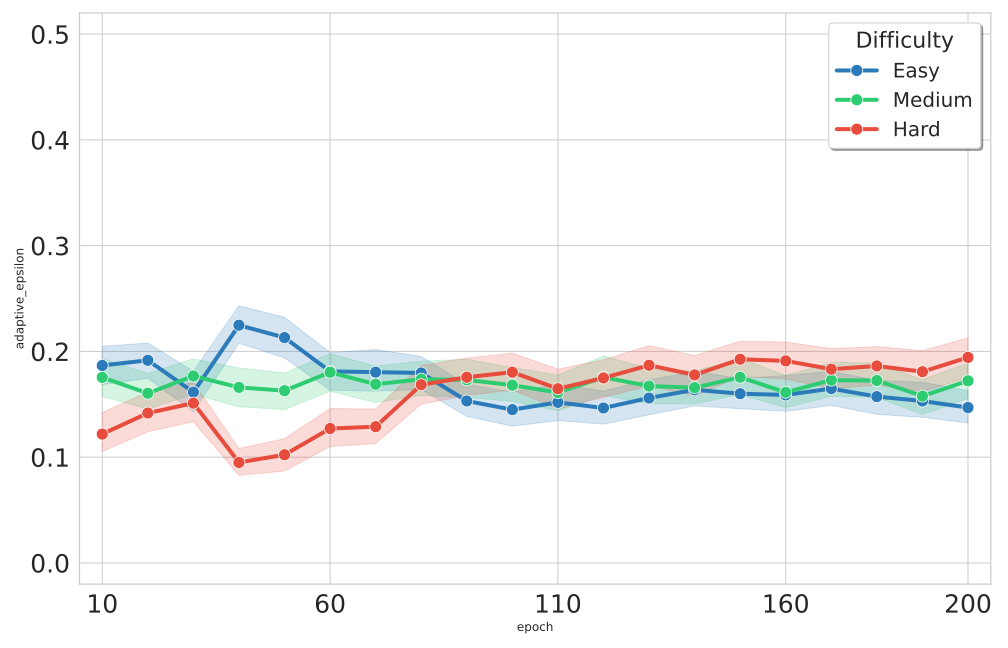
\includegraphics[width=\linewidth]{figure/epsilon_combined_lineplot_ci.pdf}
    \caption{Evolution of the adaptive parameter $\epsilon$ throughout the training process on the CVC-ClinicDB dataset. Cases are categorized into ``Easy,'' ``Medium,'' and ``Hard'' based on their baseline segmentation performance. Solid lines represent the mean values, and shaded regions denote the $99\%$ confidence intervals.}
    \label{fig:epsilon_evolution}
\end{figure}

\clearpage

\begin{figure}[t]
    \centering
    \includegraphics[width=\linewidth]{figure/difficulty_lineplot_comparison_ci99.pdf}
    \caption{Dice coefficient transitions throughout training for different difficulty levels on CVC-ClinicDB. Curves show the mean values of the proposed (red) and baseline (gray) methods, with shaded areas indicating 99\% confidence intervals.}
    \label{fig:convergence_ci99}
\end{figure}

\clearpage

\subsubsection{Impact of Hyperparameters}
In this section, we conduct a sensitivity analysis of the main hyperparameters in the proposed method to verify the validity of the design choices.

\textbf{Impact of $\epsilon$ Range:}
As shown in Table \ref{tab:ablation_epsilon_cvc} and Table \ref{tab:ablation_epsilon_kvasir-seg}, the best segmentation performance was obtained on both datasets when the variation range of $\epsilon$ was set to $[0, 0.5]$.
Expanding the upper limit $\epsilon_{\text{max}}$ from $0.3$ to $0.5$ allowed for assigning a larger $\epsilon$ to difficult cases, 
which likely appropriately emphasized the loss gradient and promoted the learning of lesion features.
On the other hand, the setting where the lower limit $\epsilon_{\text{min}}$ was extended to $-0.3$ ($\epsilon_{\text{min}}=-0.3, \epsilon_{\text{max}}=0.5$) did not improve performance compared to the case of $\epsilon_{\text{min}}=0$.
This is likely because the excessive expansion of the range increased the sensitivity to minute noise contained in the uncertainty estimation more than necessary, thereby impairing training stability.

\textbf{Impact of Sensitivity Parameter $k$:}
Table \ref{tab:ablation_k_cvc} and Table \ref{tab:ablation_k_kvasir-seg} show the results of varying the slope $k$ of the sigmoid function with respect to the difficulty score.
On the Kvasir-SEG dataset, the accuracy was highest when $k=2$. On the CVC-ClinicDB dataset, although $k=3$ showed slightly higher values, $k=2$ achieved comparable performance.
When the slope is too gentle, such as $k=1$, the difference in difficulty is not sufficiently reflected in the loss shape. Conversely, when it is too steep, such as $k=3$, the loss shape switches binarily, which may cause unstable learning.
Based on the above, it is considered that $k=2$ is an appropriate setting for balancing smooth adaptation according to difficulty and stable learning.

\textbf{Impact of the Adaptation Start Epoch $E_0$:}
As illustrated in Fig. \ref{fig:ablation_e0}, an earlier timing for the commencement of adaptive learning yielded superior results, with the highest performance recorded at the earliest setting,
$E_0 = 10$. As demonstrated in Section 4.2.3, distinct differences in the learning progress among cases are already evident during the early stages of training (see Fig. \ref{fig:convergence_ci99}).
It is considered that initiating adaptive control from this stage maximized the effect of promoting learning for unlearned cases.

\clearpage

\begin{table}[t]
    \centering
    \caption{Impact of the adaptive $\epsilon$ range $[\epsilon_{\text{min}}, \epsilon_{\text{max}}]$ on segmentation performance (CVC-ClinicDB dataset).}
    \label{tab:ablation_epsilon_cvc}
    \begin{tabular}{cccccc}
        \toprule
        $\epsilon_{\text{min}}$ & $\epsilon_{\text{max}}$ & Dice & IoU & Precision & Recall \\
        \midrule
        $0$ & $0.3$ & \textbf{0.7017} & \textbf{0.6050} & \textbf{0.7875} & \textbf{0.7234} \\
        $0$ & $0.5$ & 0.6924 & 0.5913 & 0.7827 & 0.7113 \\
        $-0.3$ & $0.5$ & 0.7000 & 0.5993 & 0.7818 & 0.7220 \\
        \bottomrule
    \end{tabular}
\end{table}

\begin{table}[t]
    \centering
    \caption{Impact of the adaptive $\epsilon$ range $[\epsilon_{\text{min}}, \epsilon_{\text{max}}]$ on segmentation performance (Kvasir-SEG dataset).}
    \label{tab:ablation_epsilon_kvasir-seg}
    \begin{tabular}{cccccc}
        \toprule
        $\epsilon_{\text{min}}$ & $\epsilon_{\text{max}}$ & Dice & IoU & Precision & Recall \\
        \midrule
        $0$ & $0.3$ & 0.8239 & 0.7391 & 0.8608 & 0.8410 \\
        $0$ & $0.5$ & \textbf{0.8272} & \textbf{0.7440} & \textbf{0.8707} & 0.8397 \\
        $-0.3$ & $0.5$ & 0.8189 & 0.7313 & 0.8537 & \textbf{0.8454} \\
        \bottomrule
    \end{tabular}
\end{table}

\begin{table}[t]
    \centering
    \caption{Sensitivity analysis of the sigmoid slope parameter $k$ in the control function (CVC-ClinicDB dataset).}
    \label{tab:ablation_k_cvc}
    \begin{tabular}{ccccc}
        \toprule
        $k$ & Dice & IoU & Precision & Recall \\
        \midrule
        $1$ & 0.6935 & 0.5962 & 0.7853 & 0.7175 \\
        $2$ & 0.6924 & 0.5913 & 0.7827 & 0.7113 \\
        $3$ & \textbf{0.7063} & \textbf{0.6084} & \textbf{0.8010} & \textbf{0.7178} \\
        \bottomrule
    \end{tabular}
\end{table}

\begin{table}[t]
    \centering
    \caption{Sensitivity analysis of the sigmoid slope parameter $k$ in the control function (Kvasir-SEG dataset).}
    \label{tab:ablation_k_kvasir-seg}
    \begin{tabular}{ccccc}
        \toprule
        $k$ & Dice & IoU & Precision & Recall \\
        \midrule
        $1$ & 0.8235 & 0.7404 & 0.8589 & \textbf{0.8440} \\
        $2$ & \textbf{0.8272} & \textbf{0.7440} & \textbf{0.8707} & 0.8397 \\
        $3$ & 0.8229 & 0.7375 & 0.8663 & 0.8370 \\
        \bottomrule
    \end{tabular}
\end{table}

\begin{figure}
    \centering
    \includegraphics[width=\linewidth]{figure/fig_E0_effect.pdf}
    \caption{Effect of adaptation start epoch $E_0$ on segmentation performance (Dice coefficient) for the CVC-ClinicDB (left) and Kvasir-SEG (right) datasets. }
    \label{fig:ablation_e0}
\end{figure}

\clearpage

\subsubsection{Qualitative Evaluation}
Fig. \ref{compare} shows the segmentation results of the comparative methods and the proposed method for representative cases of each difficulty level in the CVC-ClinicDB dataset.
For easy and medium cases where the boundaries are clear, both existing methods and the proposed method achieve high-precision segmentation.
On the other hand, in difficult cases where the contrast between the polyp and the mucosal wall is low and the boundaries are unclear,
the baseline Dice Loss and Focal Loss failed to capture the polyp region, resulting in significant under-detection. Even PolyDice-1 Loss (optimal) shows incomplete detection.
In contrast, the proposed method appropriately captures the polyp boundaries and achieves good segmentation results.
This result suggests that the proposed method determined the case as a difficult image via MC Dropout and set a large shape parameter $\epsilon$ for the loss function,
thereby strengthening the gradient during training and improving the feature extraction capability in low-contrast regions.

\begin{figure*}[t]
    \centering % 図を中央揃えにする(推奨)
    \includegraphics[width=\linewidth]{figure/compare.pdf}
    \caption{Qualitative comparison of segmentation results on the CVC-ClinicDB dataset. Each row represents a different difficulty level (easy, medium, hard), categorized by baseline Dice Loss performance.}
    \label{compare}
\end{figure*}